\section{Wikipediaで6回リンクたどればいけるか調べるサイトを一日で作った話}
\subsection{概要}
暑いですね。
これを書いている今日は7/1ですが、皆さんいかがお過ごしでしょうか。

初めまして、\htmladdnormallinkfoot{@mtgto}{http://twitter.com/mtgto}です。ふだんは会社でiPhoneアプリやHTTPサーバのプログラムを書いて過ごしています。

昨年の今頃、私はとあるSNSサービスの新規立ち上げの開発に携わっており、土日があったりなかったりという程度の忙しさに巻き込まれていました。
ちょうどその頃は仕事も佳境にきており、私の仕事は品質保証テストで上がってきた問題の解決を行うということがほとんどでした。
職業上仕方がないことなのですが、家に帰って寝るだけの日々に辟易していました。
そんな折に「\htmladdnormallinkfoot{wikipediaは6回リンクを辿ればどのページでもいけるらしいwww}{http://blog.livedoor.jp/goldennews/archives/51657545.html}」という記事をRSSリーダーで見かけました。

私がこの記事を読んだ時に、ふと「これって自動で見つけられるのかな」と思ったところからこの話は始まります。

なお3分クッキングよろしく\htmladdnormallinkfoot{実際に完成したサイト}{http://pediaroute.com/}がありますので、探索の仕組みやら作った時の苦労話に興味が無い方は読み飛ばしていただいて構いません。
お手数ですが右上の×ボタンを押して閉じてください。

例えば「おはよう」から「おやすみ」までをpediarouteで検索すると、
\begin{figure}
  \centering
  \fbox{
    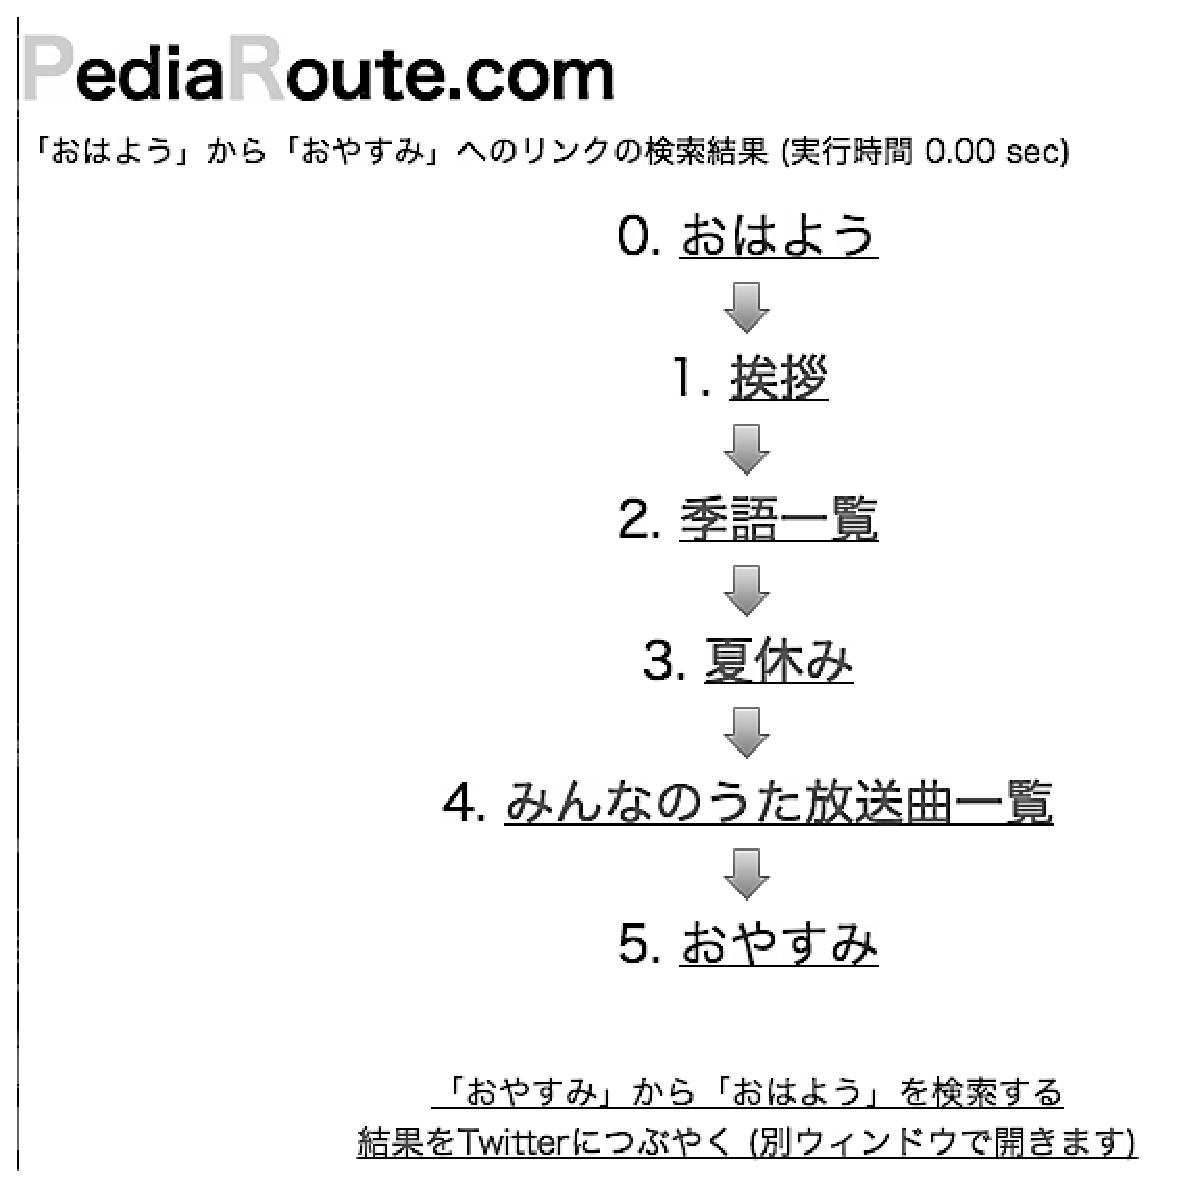
\includegraphics[width=9cm,clip]{goto-pedia/img/ohayou-oyasumi.eps}
  }
  \caption{pediarouteでおはようからおやすみを検索したところ}
\end{figure}
探索時間0.00秒以内(10ミリ秒以内は切り捨て)で「おはよう」→「挨拶」→「季語一覧」→「夏休み」→「みんなのうた放送曲一覧」→「おやすみ」という解答を見つけることができます。

\subsection{設計}
知人の知人というように辿って行くとわずか6回辿るだけで世界中の人間に辿り着けるという話を聞いたことがあるでしょうか?

これはいわゆる「\htmladdnormallinkfoot{六次の隔たり}{http://ja.wikipedia.org/wiki/\%E5\%85\%AD\%E6\%AC\%A1\%E3\%81\%AE\%E9\%9A\%94\%E3\%81\%9F\%E3\%82\%8A}」というもので、
詳細はWikipediaなどに丸投げしちゃいますが、知り合いの知り合いの知り合い〜というように知り合いをつてに辿って行くと6人いれば全ての人に到達できるというものです。

例えば、私の知人にビル・ゲイツと知り合いという人がいるので、私からビル・ゲイツまでは3ホップで辿り着けることとなります。

そもそもWikipediaのリンクの最短検索ということが現実的に可能なのでしょうか?まずはそれを検討することにしました。
※ここでいう現実的に可能とは、ウェブサイトとして負荷に耐えられるかどうかも含みます。

まずは具体的な数値データを知るためにデータのダウンロードを行いましょう。
Wikipediaのページデータやリンク、画像などは「\htmladdnormallinkfoot{データベースダウンロード}{http://ja.wikipedia.org/wiki/Wikipedia:\%E3\%83\%87\%E3\%83\%BC\%E3\%82\%BF\%E3\%83\%99\%E3\%83\%BC\%E3\%82\%B9\%E3\%83\%80\%E3\%82\%A6\%E3\%83\%B3\%E3\%83\%AD\%E3\%83\%BC\%E3\%83\%89}」からダウンロードすることができます。
今回必要なのはページデータ(page.sql.gz)とページ間リンクデータ(pagelinks.sql.gz)の2つだけです。この中にはMySQLのクエリの塊が入っています。

2011年8月当時は30kB/秒ほど出なかったので、ダウンロードを開始してから寝た覚えがありますが、
2012年7月に最新版(20120630)をダウンロードしてみたところ300kB/秒ほど出るようになっていました。界王拳10倍だ!

Wikipediaのページ数は204万件(2011年8月24日版)、ページ間のリンクの数は6,677万件ありました。リンクの数は多いページで平均すると00を超える程度でしょう。
ちなみにリンク数が最大のページは「\htmladdnormallinkfoot{化学に関する記事の一覧}{http://ja.wikipedia.org/wiki/化学に関する記事の一覧}」で、ページ内のリンクが6,523もあります。

今回の問題をプログラミングの問題っぽく表現すると、
\begin{itembox}{問題}
ページをノード、ページ間のリンクを枝(枝の長さはすべて長さ1とする)とした巨大な有向グラフがある。

この有向グラフと特定の始点ノードと終点ノードがあたえられたときに、
有向グラフ上の長さ6以下で到達できる最短の経路を求めよ。
\end{itembox}
というものになります。

プログラムでの探索手順としては有名なものに「深さ優先探索」と「幅優先探索」があります。有名すぎるので知らない人はぐぐってください。
最短のものを見つけることを必要としないのであれば、それ以外にも
今回は最大の深さを6とした深さ優先探索(もしくは反復深化深さ優先探索)と
つまりページ数xページ数のリンクがあるかどうかのテーブルを作らずとも

設計段階ではしょりましたが、ダイクストラ法などを利用してもよいと思います。
その場合にはノードとノードの距離がどれも1として行えばOKです(幅優先探索と変わらなくなりますが)。

今回は始点ノードと終点ノードからそれぞれ幅優先探索を行い、最初に両側からの探索で見つかったものを採用することにしました。

\begin{itembox}{双方向からの幅優先探索}
始点ノードから到達できるノード集合をS、終点ノードへと到達できるノード集合をGとする
\begin{enumerate}
\item 探索の初期状態は、
\[
S_0 = {N_S}, G_0 = {N_G}
\]
となっている
\item 集合SとGのどちらか小さい方から一つだけ探索を行う。
  \begin{enumerate}
    \item Sが小さい場合はSに含まれるノードから一つだけリンクを行ったノードを求め(どのノードから探索されたかをメモっておく)、それぞれがGに含まれるかどうかを調べる。
      このノードがGに含まれる場合は経路が見つかったのでメモしておいたリンク元(先)ノード情報から経路を求める。
    \item Gが小さい場合はGに含まれるノードから一つだけ逆リンクを行ったノードを求め(どのノードから逆探索されたかをメモっておく)、それぞれがSに含まれるかどうかを調べる。
      このノードがSに含まれる場合は経路が見つかったのでメモしておいたリンク先(元)ノード情報から経路を求める。
  \end{enumerate}
\item 見つからなければ2. に戻る。5回探索しても見つからなかったらリンクがないと返す。
\end{enumerate}
\end{itembox}
\begin{figure}
  \centering
  \fbox{
    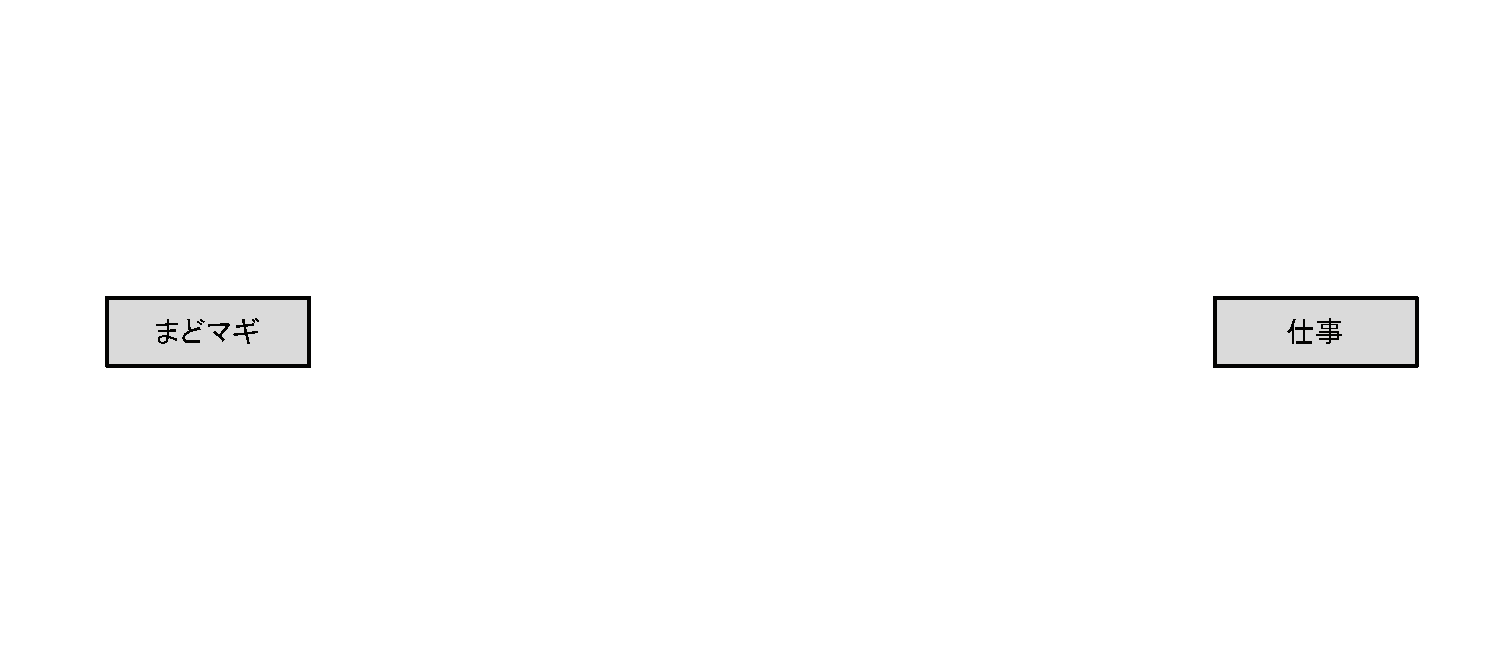
\includegraphics[width=9cm,clip]{goto-pedia/img/pediaroute01.eps}
  }
  \fbox{
    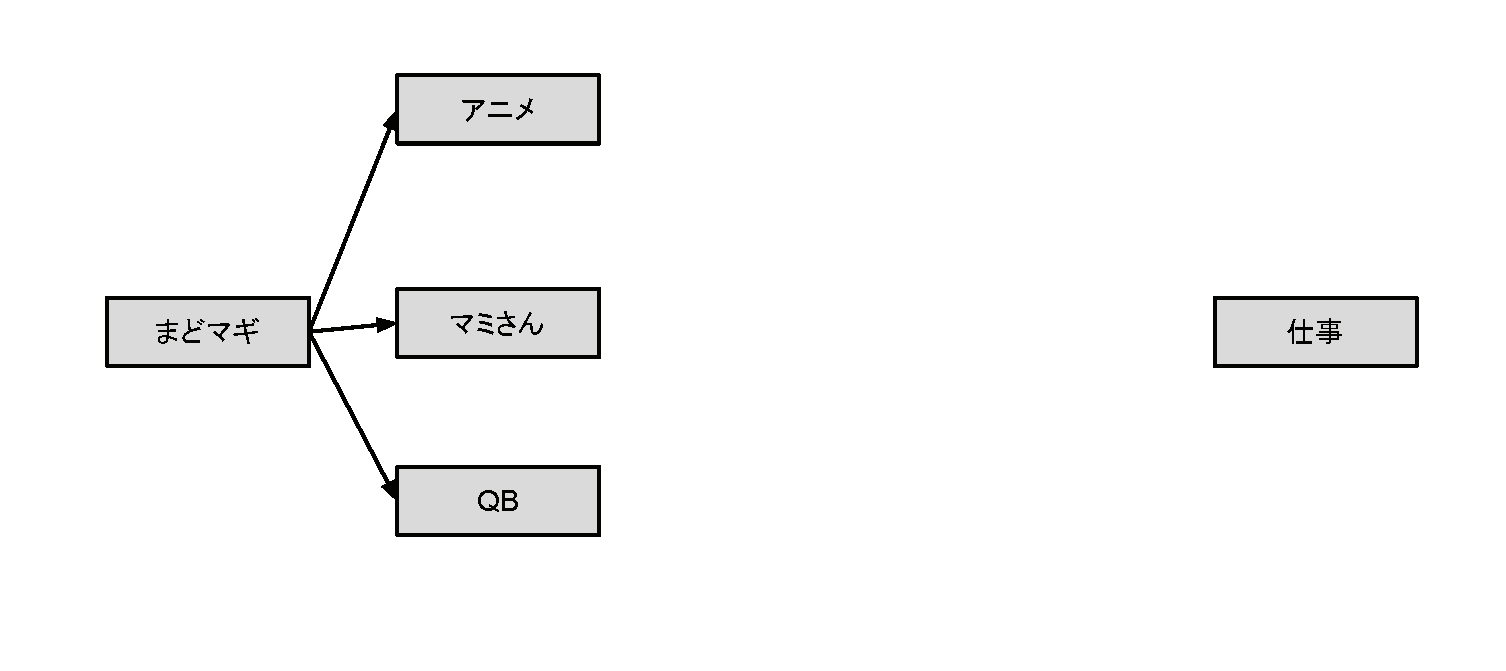
\includegraphics[width=9cm,clip]{goto-pedia/img/pediaroute02.eps}
  }
  \fbox{
    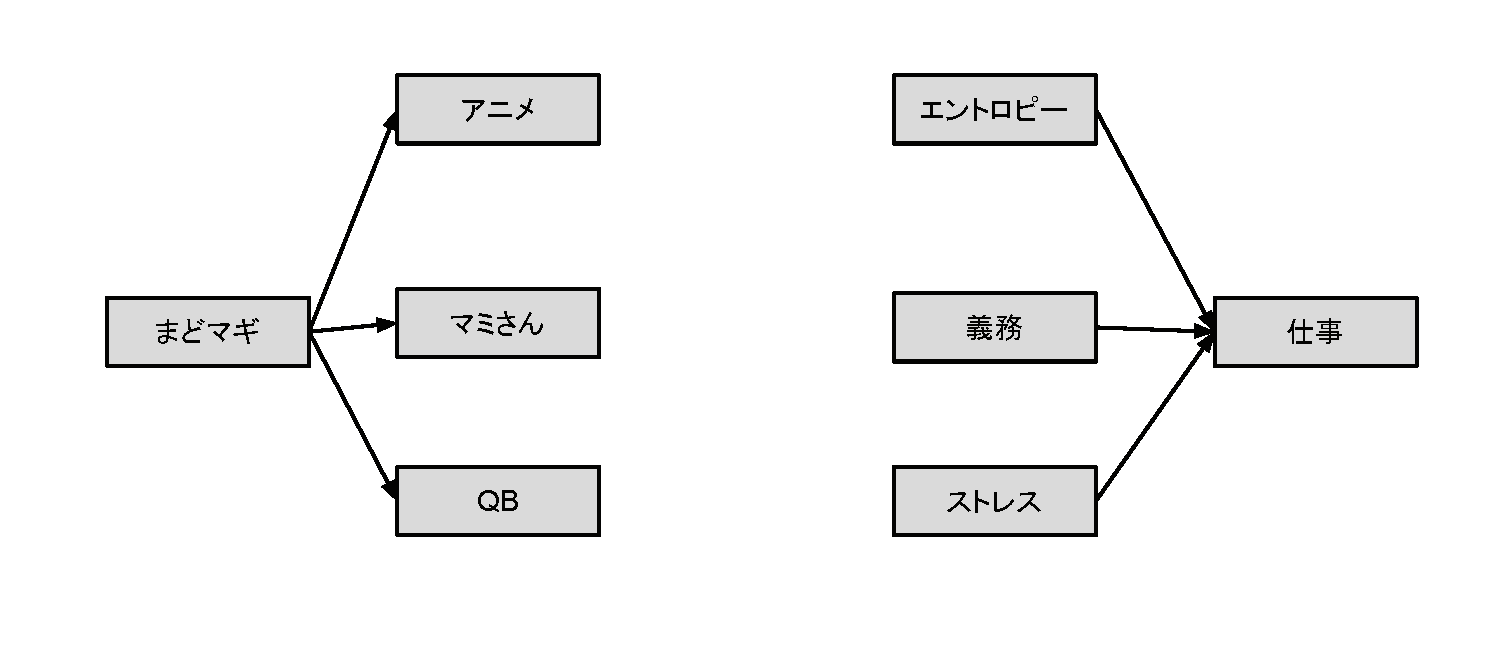
\includegraphics[width=9cm,clip]{goto-pedia/img/pediaroute03.eps}
  }
  \fbox{
    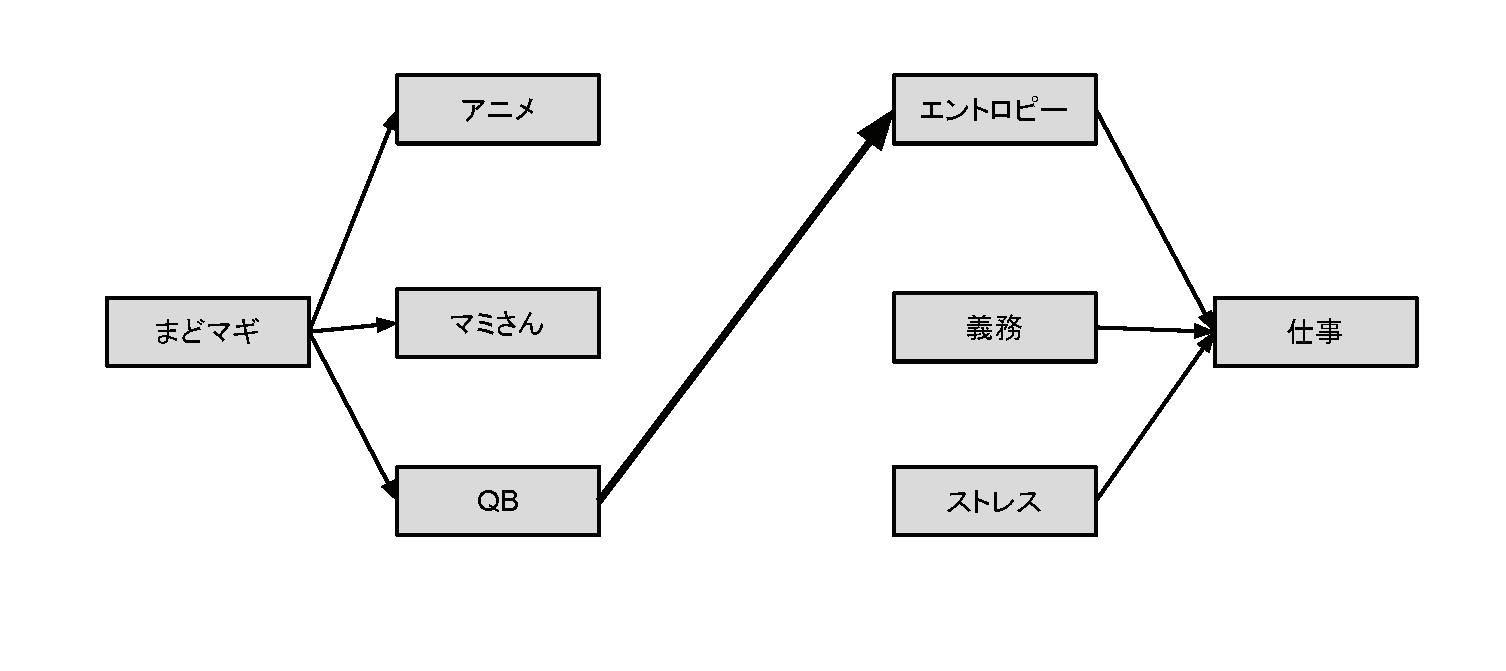
\includegraphics[width=9cm,clip]{goto-pedia/img/pediaroute04.eps}
  }
  \caption{探索の例}
\end{figure}

\subsubsection{使用言語の選択}
今回の設計ではすべてのリンクをメモリ上におかなければなりません。
このため1リンクごとに消費されるサイズがなるべく小さいことが望まれます
\footnote{ページ数が256*256*256以下なら3バイト表現にするのですが、日本のWikipediaのページは200万以上あったのでおとなしく4バイトにしました}。
動的言語ではメモリの消費量を見積もることが難しかったので、今回はコンパイル言語の中でJava、C、C++が残り、開発するために残された時間の短さの制約から普段から書き慣れているJavaを選択しました。

\subsection{IRCボット完成まで}
さて設計が完成したので実装をはじめることにしましょう。
実装の工程は大きく分けて
\begin{itemize}
\item ページデータとリンクデータをメモリ上に乗せやすい形に変換する
\item メモリ上にあるページデータとリンクデータを使って探索を行う
\end{itemize}
の2つです。

\subsubsection{ページデータとリンクデータの作成}
ページデータ、ページ間のリンクデータはMySQLのSQLクエリとして提供されています。
SQLクエリとはいえ、ただのINSERT文(リンクデータの場合3000万行ありますが)あるだけですので、
もちろん正規表現などを使用して読み込んでも構わないのですが、
今回は実装に時間がないことから(そればっかり)確実さを重視して一度MySQLへのインポートを行なってから処理することにしました。
今回の開発はすべてMacBook Airで行いましたが、ローカルのMySQL (5.5.x) にインポートを完了するのにも2時間半かかりました。
その間に小さいモデルでの探索プログラムの開発をしていればよかったんですが、

ちなみに今回はページデータとリンクデータのみを利用しましたが、それ以外にも様々なデータが提供されています。
例を挙げると、

\subsubsection{探索}
探索プログラムは先に出てきた「両側からの幅優先探索」を行うものです。
まず用意したデータからページ間のリンク(リンク先とリンク元の両方を用意したので、通常の二倍使用しています)をメモリ上に展開します。
最初は手で紙に書いた小さなグラフで実装、デバッグを行い、そのあと実際のデータを使って確認を行いましたが
小さなグラフでちゃんと探索できるようになったあとはほぼバグもなくスムーズに進めることが出来ました。

\subsubsection{IRC Bot}
まずIRCの仲間たちにお披露目するためにIRC botとして作ることにしました。
IRCを簡単に説明すると複数人と同時にオンラインチャットできるシステムです。
今回IRCへの接続、ボット処理(誰かの発言に対してプログラムが発言を返したりすること。人工無脳が有名)には
\htmladdnormallinkfoot{PircBot}{http://www.jibble.org/pircbot.php/}を使い、
誰かの''w:ドラえもん 野球''という発言に対して、''$[$ドラえもん, 野球$]$ ドラえもん -$>$ 1940年 -$>$ 野球''を返してくれるプログラムを作成しました。
IRCボットが完成したのが21時22分のことでした。

\begin{itembox}{その日のirc ログ}
  21:22:02 $<$mtgto$>$ w: 花火 出店\\
  21:22:03 {goto\_bot} [花火, 出店] 花火 -$>$ 飯田市 -$>$ リンゴ -$>$ 出店 (0.02sec)\\
  21:22:07 $<$mtgto$>$ やっとできた\\
  21:22:19 * ***** changed mode (+o, goto\_bot)\\
  21:22:34 $<$mtgto$>$ w: ドラえもん 野球\\
  21:22:35 {goto\_bot} [ドラえもん, 野球] ドラえもん -$>$ 1940年 -$>$ 野球 (0.00sec)\\
  21:22:55 $<$mtgto$>$ wikipediaページリンクでいけるかな?をつくった
\end{itembox}

\subsection{Webサイト作ることにした}
この時点ではWebサーバを作成しようとは考えていなかったのですが、
友人からのIRC上でのすすめもあり、公開できるものを作ってみようと考えました。

まずはサーバから。今回のプログラムを動かすのに一番ネックになるのは実行に必要な700MB強のメモリです。
サーバはServersMan VPSの2GBプランを選択し、Ubuntu Server 10.04に適当に設定を加え(sshd、firewallくらい)Playを適当にデプロイしました。
今回はMySQLもApacheも使わないし、あっという間に終わりました。

\subsubsection{Play! framework}
探索プログラム、IRCbotをJavaによって記述したので、ウェブサーバもJavaで作ることにしました。
残り時間が限られているため、簡単に使えるウェブフレームワークを探したところ、
\htmladdnormallinkfoot{Play! framework}{http://playframework.org/}がいいのではないかと判断しました。
TomcatとかJettyとかはウェブサーバとしてはもちろん「強い」のですが、即日公開したいサービスには巨大すぎました・・・。

Play!はRuby on rails風のMVCウェブサーバで、Javaで記述することができます。
railsはそれなりに使ったことがあったのも良かったのかもビューテンプレートが独自で、さらにビューへの引数の型が要求されるなどrailsとは違った苦労もありましたが
デプロイは非常に簡単で便利ですね。
実際Play!を使ったのは今回が初めてでしたが、それほど戸惑うことなく(検索画面と検索結果の2ページしかないしょっぽいウェブサイトですが)サクサク作ることができました。

\subsubsection{ドメインとったよ}
最初は自分が普段使っているサイトのサブドメインで運用していたのですが、仲間の助言もあり、せっかくだし専用のドメインにするかと思い、pediaroute.comを取りました。

\subsubsection{負荷ヤバイの話}
公開した初日はIRCのメンバーと自身のツイッターでつぶやいた程度だったため、全然流行らず作っただけの自己満で終わるところでした。
それが会社内でのIRCで宣伝したところ、それなりに口コミで流行し、最大で秒間10回程度のアクセスが発生するほどになりました。

会社内からそれを見て喜んでいたのですが、一方で「つながらない」というコメントも見受けられるようになり、
実際にアクセスしてみると検索はおろかページの表示すらままならないということに気づきました。

調べたところ、今回探索を行う処理を「synchronizedブロックを使って」最大1スレッドまでとしているのですが、
(これには理由があって探索処理はCPUはそれほど食わないのですがメモリを多い時に数メガバイト持っていくので、
 同時に探索を許可してしまうとメモリの上限を超えて、Java VMがクラッシュしてしまう危険性があったため規制していました。)
このロックとPlay!のりクエスト処理の相性が悪かったようで、その後Promiseという仕組みを使って書き直したところ落ちることはなくなりました。
身を持って慣れてないウェブフレームワークを使うことの難しさを再考させられる経験になりました。

\subsubsection{そのあと}
そのあとはちょいとある程度まともなデザインに仕上げたりしましたが、仕事が忙しいのと(そればっかり)飽きたのもあり、特に話題にもならず、ひっそりと忘れ去られて行きました。
いや、まだあるけどね!この原稿をあなたが手にとっているときにまだサービス続けてるけどね!
広告もつけてないから続ければ続けるほど損するシステムなんだけどね!

wikitterの中の人とtwitterでやり取りしたりもしましたが、内容はないしょにしておきます。

\subsection{まとめ、今後の予定}
pediarouteの話はどこかで書こうと思っていたのですが、こういう形で過去の創作物の話をまとめることができて幸いでした。
当時は「コーディング・ハイ」という感じで、だれることなくフルスピードでプログラムを仕上げることができ、とても楽しかったのをよく覚えています。
気が向いたら英語版も作ってみたいですね(またデスマに巻き込まれた時にでも・・・)。
